\scanpage{11}
% archive foliation: 10
\begin{center}
U N I V E R S I T E\\
DES SCIENCES ET TECHNIQUES\\
DU LANGUEDOC\\
\texttt{-{}-{}-{}-{}-{}-{}-{}-{}-{}-{}-{}-{}}

Service de la Scolarité\\
MA / GJ\\
Diffusion : Liste A\\
N° : 3547
\end{center}

MONTPELLIER, le 19 JUIN 1981

AVIS DE SOUTENANCE D'UN \unsure{DIPLOME|DIPLÔME} D'ETUDES SUPERIEURES D'UNIVERSITE

\texttt{-{}-{}-{}-{}-{}-{}-{}-{}-{}-{}-{}-{}-{}-{}-{}-{}-{}-{}-{}-{}-{}-{}-{}-{}-{}-{}-{}-{}-{}-{}-{}-{}-{}-{}-{}-{}-{}-{}-{}-{}-{}-{}-{}-{}-{}-{}-{}-{}-{}-{}-{}-{}-{}-{}-{}-{}-{}-{}-{}-{}-{}-{}-{}-{}-{}}

Le 30 JUIN 1981 à 16 heures 30 mn

A L'ECOLE NATIONALE SUPERIEURE DE CHIMIE\\
(Amphi Gerhard)

Monsieur EL MANSOURI Abdeslam

soutiendra un Diplôme d'Etudes Supérieures d'Université portant sur le sujet suivant :

``Contribution à l'étude des systèmes binaires $\mathrm{PbF}_2$ - $\mathrm{SnF}_4$ et $\mathrm{PbF}_2$ - $\mathrm{GeF}_4$''.

\uline{Membres du jury} :
\begin{tabular}{ll}
MM.&COT L.\\
&RIBES M.\\
&LIVAGE L.\\
&GRANIER W.\\
&VIMINOT S.
\end{tabular}

P. le Secrétaire Général,\\
l'Attachée d'Administration Universitaire,

\unsure{Gentil}
\figure{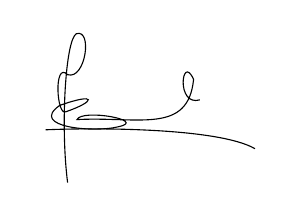
\begin{tikzpicture}[x=1cm,y=1cm]
\draw (0.2,-0.55) .. controls (0.11,0.15) and (0.17,1.25) .. (0.31,1.34)
.. controls (0.52,1.41) and (0.43,0.75) .. (0.20,0.82)
.. controls (0.02,1.00) and (0.06,0.28) .. (0.18,0.35)
.. controls (0.56,0.48) and (0.58,0.60) .. (0.10,0.43)
.. controls (-0.30,0.15) and (0.55,0.08) .. (0.85,0.16)
.. controls (1.22,0.24) and (0.38,0.39) .. (0.32,0.25)
.. controls (1.11,0.29) and (1.73,0.06) .. (1.80,0.76)
.. controls (1.65,1.10) and (1.57,0.41) .. (1.88,0.50);
\draw (-0.08,0.12) .. controls (0.62,0.15) and (2.13,0.14) .. (2.58,-0.12);
\end{tikzpicture}}
A. GENTIL
